\documentclass[10pt]{article}
\usepackage[a4paper,landscape,margin=3.4mm]{geometry}
\usepackage[T1]{fontenc}
\usepackage{lmodern}
\usepackage{tikz}
\usetikzlibrary{arrows.meta}
\usepackage{xcolor}
\pagestyle{empty}
\setlength{\parindent}{0pt}
\setlength{\parskip}{0pt}

\definecolor{sense}{RGB}{14,90,166}
\definecolor{comp}{RGB}{158,82,6}
\definecolor{outp}{RGB}{18,108,54}
\definecolor{pwr}{RGB}{70,70,70}

\tikzset{
  S/.style={draw=sense, fill=sense!9, line width=0.32pt,
            font=\fontsize{4.7}{5.2}\selectfont\bfseries,
            inner sep=1.15pt, rounded corners=0.45pt, align=center, text=sense!75!black},
  C/.style={draw=comp, fill=comp!11, line width=0.32pt,
            font=\fontsize{4.7}{5.2}\selectfont\bfseries,
            inner sep=1.15pt, rounded corners=0.45pt, align=center, text=comp!80!black},
  O/.style={draw=outp, fill=outp!10, line width=0.32pt,
            font=\fontsize{4.7}{5.2}\selectfont\bfseries,
            inner sep=1.15pt, rounded corners=0.45pt, align=center, text=outp!75!black},
  P/.style={draw=pwr, fill=black!5, line width=0.28pt,
            font=\fontsize{4.5}{5}\selectfont,
            inner sep=1.05pt, rounded corners=0.45pt, align=center, text=pwr},
  box/.style={draw=black!60, line width=0.38pt, rounded corners=0.6pt},
  arr/.style={-{Stealth[length=1.25mm,width=0.95mm]}, line width=0.42pt, black!70},
  lbl/.style={font=\fontsize{4.15}{4.6}\selectfont, text=black!72, inner sep=0.5pt, align=center}
}

\newcommand{\sw}[2]{\tikz[baseline=-0.5ex]\draw[#1,fill=#1!10,line width=0.35pt] (0,0) rectangle (2mm,1.6mm);\,#2}

\newcommand{\cell}[3]{%
\begin{minipage}[t]{0.474\textwidth}
{\fontsize{6.35}{7.2}\selectfont\bfseries #1}\par
#2\par\vspace{0.15mm}
{\fontsize{4.85}{5.7}\selectfont #3}
\end{minipage}}

\begin{document}
\vspace*{-0.6mm}
{\fontsize{8.6}{9.6}\selectfont\bfseries MSL prior-art sheet --- component cross-sections and signal order}\hfill
{\fontsize{5}{5.6}\selectfont \sw{sense}{sense}\ \sw{comp}{compute}\ \sw{outp}{output}\ \sw{pwr}{power}}\\[0.2mm]
{\fontsize{4.55}{5.3}\selectfont\color{black!68}%
One A4 sheet, landscape. Original schematics of published layouts, not copies of patent figures. Left column: products. Right column: patents. Arrows are the signal order along the device. SmartCane and IN~1354/DEL/2007 are related and are not the same unit.}
\vspace{0.9mm}

\noindent
\cell{1 \quad Oculosense Drishti Vision \textnormal{\fontsize{4.6}{5}\selectfont --- glasses, 49\,g}}
{%
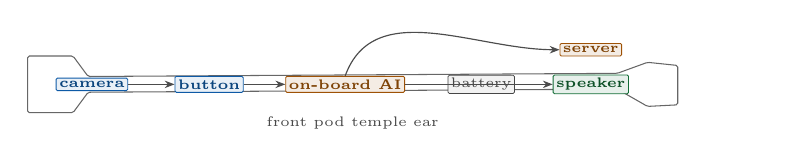
\begin{tikzpicture}[x=0.96mm,y=1mm]
  \draw[box] (0,1.6) -- (6,1.6) -- (8,4.2) -- (78,4.6) -- (82,2.4) -- (86,2.6) -- (86,7.6) -- (82,8.0) -- (78,6.6) -- (8,6.2) -- (6,8.8) -- (0,8.8) -- cycle;
  \node[S] (cam) at (8.5,5.2) {camera};
  \node[S] (btn) at (24,5.2) {button};
  \node[C] (ai) at (42,5.2) {on-board AI};
  \node[P] at (60,5.2) {battery};
  \node[O] (spk) at (74.5,5.2) {speaker};
  \node[C] (cld) at (74.5,9.6) {server};
  \draw[arr] (cam) -- (btn);
  \draw[arr] (btn) -- (ai);
  \draw[arr] (ai) -- (spk);
  \draw[arr] (ai.north) to[out=70,in=180] (cld.west);
  \node[lbl,anchor=north] at (43,1.3) {front pod \hfill temple \hfill ear};
\pgfresetboundingbox\useasboundingbox (0,-0.2) rectangle (97,12.4);\end{tikzpicture}%
}
{Button or voice, then the camera, then on-board AI. Wi-Fi or Bluetooth also reaches the Oculosense server (Gemini). The built-in speaker returns text, scene, face, and direction with distance. No phone in the hand.}
\hfill
\cell{1 \quad IIT Delhi --- IN 1354/DEL/2007 \textnormal{\fontsize{4.6}{5}\selectfont --- unit on one cane fold}}
{%
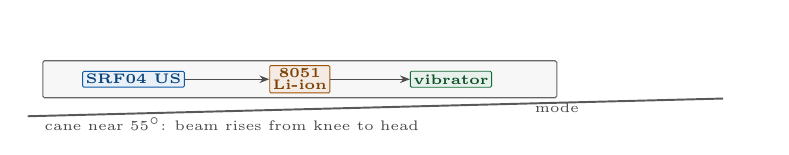
\begin{tikzpicture}[x=0.96mm,y=1mm]
  \draw[box,fill=black!3] (2,3.5) rectangle (70,8.2);
  \node[S] (us) at (14,5.85) {SRF04 US};
  \node[C] (mcu) at (36,5.85) {8051\\[-0.3mm]Li-ion};
  \node[O] (vib) at (56,5.85) {vibrator};
  \node[lbl] at (70,2.3) {mode};
  \draw[line width=0.7pt,black!65] (0,1.15) -- (92,3.4);
  \node[lbl,anchor=west] at (2,0.15) {cane near \(55^\circ\): beam rises from knee to head};
  \draw[arr] (us) -- (mcu);
  \draw[arr] (mcu) -- (vib);
\pgfresetboundingbox\useasboundingbox (0,-0.2) rectangle (97,12.4);\end{tikzpicture}%
}
{Echo time to the 8051, then a cellphone vibrator. The rate rises as the obstacle closes. Short mode is under 1\,m with 3 patterns; long mode has 4. The cane tip, not this unit, still finds the ground.}

\vspace{0.15mm}
\noindent
\cell{2 \quad OrCam MyEye 2 Pro \textnormal{\fontsize{4.6}{5}\selectfont --- clip, \(76\times 21\times 15\)\,mm}}
{%
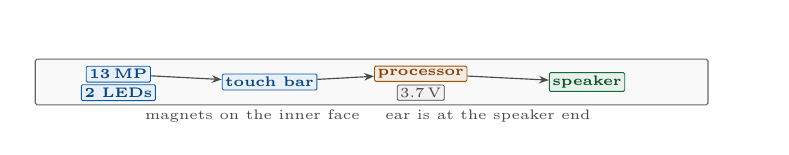
\begin{tikzpicture}[x=0.96mm,y=1mm]
  \draw[box,fill=black!2.5] (1,2.6) rectangle (90,8.4);
  \node[S] (cam) at (12,6.5) {13\,MP};
  \node[S] at (12,4.15) {2 LEDs};
  \node[S] (bar) at (32,5.5) {touch bar};
  \node[C] (cpu) at (52,6.55) {processor};
  \node[P] at (52,4.15) {3.7\,V};
  \node[O] (spk) at (74,5.5) {speaker};
  \draw[arr] (cam) -- (bar);
  \draw[arr] (bar) -- (cpu);
  \draw[arr] (cpu) -- (spk);
  \node[lbl] at (45,1.15) {magnets on the inner face \quad ear is at the speaker end};
\pgfresetboundingbox\useasboundingbox (0,-0.2) rectangle (97,12.4);\end{tikzpicture}%
}
{Point, tap, or voice captures one frame. Offline OCR, face, barcode, colour, and product run inside the clip. Audio leaves the speaker, or Bluetooth. Wi-Fi is for updates only. MyEye 2 has no belt pack.}
\hfill
\cell{2 \quad Snap --- US 11,215,846 B1 \textnormal{\fontsize{4.6}{5}\selectfont --- lights and bridge haptics}}
{%
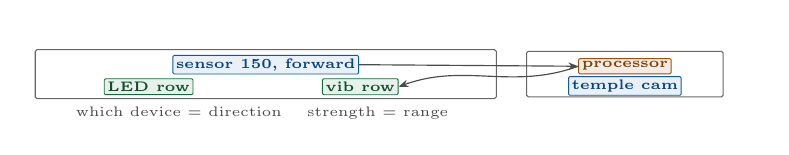
\begin{tikzpicture}[x=0.96mm,y=1mm]
  \draw[box] (1,3.4) rectangle (62,9.6);
  \node[S] (sen) at (31.5,7.7) {sensor 150, forward};
  \node[O] (led) at (16,4.9) {LED row};
  \node[O] (vib) at (44,4.9) {vib row};
  \draw[box] (66,3.6) rectangle (92,9.4);
  \node[C] (cpu) at (79,7.5) {processor};
  \node[S] at (79,5.0) {temple cam};
  \draw[arr] (sen.east) -- (cpu.west);
  \draw[arr] (cpu.west) to[out=200,in=20] (vib.east);
  \node[lbl] at (31,1.5) {which device = direction \quad strength = range};
\pgfresetboundingbox\useasboundingbox (0,-0.2) rectangle (97,12.4);\end{tikzpicture}%
}
{The phased array returns angle and distance. Which lamp, or which vibrator on the bridge, is the direction. Brightness or vibration strength is closeness. Lights serve partial sight; haptics serve little or no sight.}

\vspace{0.15mm}
\noindent
\cell{3 \quad Envision Glasses \textnormal{\fontsize{4.6}{5}\selectfont --- Glass Enterprise Edition 2}}
{%
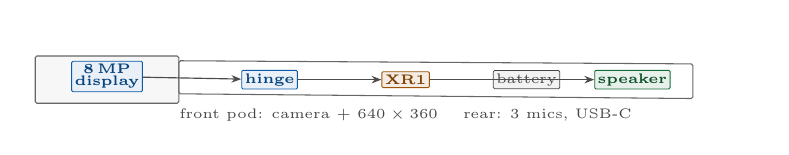
\begin{tikzpicture}[x=0.96mm,y=1mm]
  \draw[box,fill=black!3] (1,2.8) rectangle (20,8.8);
  \node[S] (cam) at (10.5,6.2) {8\,MP\\[-0.3mm]display};
  \draw[box] (20,4.0) -- (88,3.4) -- (88,7.8) -- (20,8.2) -- cycle;
  \node[S] (hng) at (32,5.8) {hinge};
  \node[C] (xr) at (50,5.8) {XR1};
  \node[P] at (66,5.8) {battery};
  \node[O] (spk) at (80,5.8) {speaker};
  \draw[arr] (cam) -- (hng);
  \draw[arr] (hng) -- (xr);
  \draw[arr] (xr) -- (spk);
  \node[lbl] at (50,1.3) {front pod: camera + \(640\times360\) \quad rear: 3 mics, USB-C};
\pgfresetboundingbox\useasboundingbox (0,-0.2) rectangle (97,12.4);\end{tikzpicture}%
}
{The camera feeds the Snapdragon XR1 in the right temple: OCR, objects, faces, scene. A directional mono speaker answers. The display can stay off. Wi-Fi is for calling a companion, not for ordinary reading.}
\hfill
\cell{3 \quad US 2021/0390882 A1 \textnormal{\fontsize{4.6}{5}\selectfont --- geometric hazards, Snap}}
{%
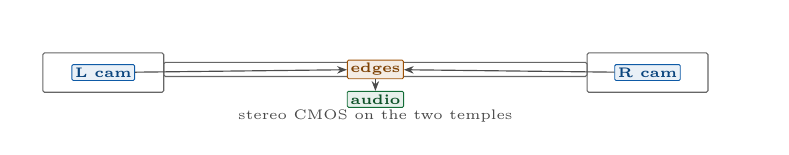
\begin{tikzpicture}[x=0.96mm,y=1mm]
  \draw[box] (2,4.2) rectangle (18,9.2);
  \draw[box] (74,4.2) rectangle (90,9.2);
  \draw[box] (18,6.2) rectangle (74,8.0);
  \node[S] (L) at (10,6.7) {L cam};
  \node[S] (R) at (82,6.7) {R cam};
  \node[C] (cpu) at (46,7.1) {edges};
  \node[O] (au) at (46,3.3) {audio};
  \draw[arr] (L) -- (cpu);
  \draw[arr] (R) -- (cpu);
  \draw[arr] (cpu) -- (au);
  \node[lbl] at (46,1.15) {stereo CMOS on the two temples};
\pgfresetboundingbox\useasboundingbox (0,-0.2) rectangle (97,12.4);\end{tikzpicture}%
}
{Both cameras feed an edge and geometry pass: presence, distance, and a coarse type. The alert is sound. This is not the LED and vibrator array of US 11,215,846. Less computation is the point, so the battery lasts longer.}

\vspace{0.15mm}
\noindent
\cell{4 \quad WeWALK Smart Cane 2 \textnormal{\fontsize{4.6}{5}\selectfont --- electronics in the handle}}
{%

\begin{tikzpicture}[x=0.96mm,y=1mm]
  \draw[box,fill=black!3] (8,3.6) rectangle (86,8.8);
  \node[S] (us) at (20,6.9) {US ToF};
  \node[O] (hap) at (40,6.9) {2 haptics};
  \node[O] (spk) at (60,6.2) {speaker};
  \node[S] at (78,6.2) {touch};
  \draw[arr] (us) -- (hap);
  \draw[arr] (hap) -- (spk);
  \node[C] at (46,1.35) {phone via BT: GPS and transit};
\pgfresetboundingbox\useasboundingbox (0,-0.2) rectangle (97,12.4);\end{tikzpicture}%
}
{A MEMS ultrasonic time-of-flight sensor looks up at chest and head, including glass and branches, then two haptics and a warning sound. GPS and transit stay on the phone and are spoken from the handle. The tip still sweeps the ground.}
\hfill
\cell{4 \quad Dotlumen --- US 12,044,541 B2 \textnormal{\fontsize{4.6}{5}\selectfont --- headset}}
{%
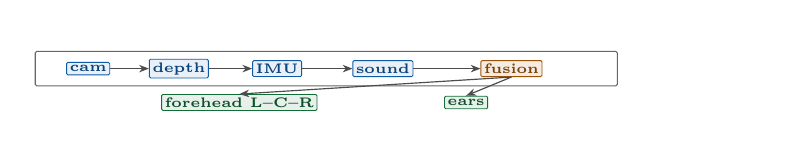
\begin{tikzpicture}[x=0.96mm,y=1mm]
  \draw[box] (1,5.0) rectangle (78,9.4);
  \node[S] (a) at (8,7.2) {cam};
  \node[S] (b) at (20,7.2) {depth};
  \node[S] (c) at (33,7.2) {IMU};
  \node[S] (d) at (47,7.2) {sound};
  \node[C] (f) at (64,7.2) {fusion};
  \node[O] (h) at (28,2.9) {forehead L--C--R};
  \node[O] (e) at (58,2.9) {ears};
  \draw[arr] (a) -- (b); \draw[arr] (b) -- (c); \draw[arr] (c) -- (d); \draw[arr] (d) -- (f);
  \draw[arr] (f.south) -- (h.north);
  \draw[arr] (f.south) -- (e.north);
\pgfresetboundingbox\useasboundingbox (0,-0.2) rectangle (97,12.4);\end{tikzpicture}%
}
{Camera, depth, IMU, and sound localisation fuse into a live map, then unconditional and conditional walkable area, then one path. Heading is the bearing to where that path cuts a circle of radius \(r\). Forehead haptics and the ears carry the cues; a virtual tunnel warns at its walls.}

\vspace{0.15mm}
\noindent
\cell{5 \quad TSAR Smart Glasses \textnormal{\fontsize{4.6}{5}\selectfont --- tsarlab.com only}}
{%
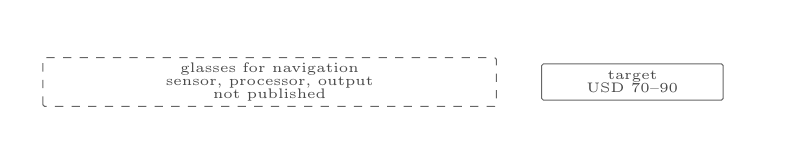
\begin{tikzpicture}[x=0.96mm,y=1mm]
  \draw[box,dashed] (2,2.4) rectangle (62,8.6);
  \node[lbl,align=center] at (32,5.5) {glasses for navigation\\sensor, processor, output\\not published};
  \draw[box] (68,3.2) rectangle (92,7.8);
  \node[lbl,align=center] at (80,5.5) {target\\USD 70--90};
\pgfresetboundingbox\useasboundingbox (0,-0.2) rectangle (97,12.4);\end{tikzpicture}%
}
{The public page gives the product class and a 70--90 dollar target, and no block diagram. Do not fill the missing chain from a different student project. Use a course handout if one was issued.}
\hfill
\cell{5 \quad InnoSpire --- US 12,440,387 B2 \textnormal{\fontsize{4.6}{5}\selectfont --- frame plus network}}
{%
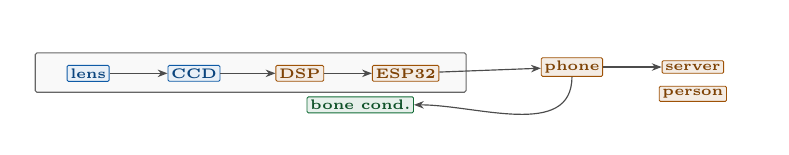
\begin{tikzpicture}[x=0.96mm,y=1mm]
  \draw[box,fill=black!2.5] (1,4.2) rectangle (58,9.2);
  \node[S] (ln) at (8,6.6) {lens};
  \node[S] (ccd) at (22,6.6) {CCD};
  \node[C] (dsp) at (36,6.6) {DSP};
  \node[C] (esp) at (50,6.6) {ESP32};
  \node[O] (bc) at (44,2.6) {bone cond.};
  \node[C] (ph) at (72,7.4) {phone};
  \node[C] (sv) at (88,7.4) {server};
  \node[C] at (88,4.0) {person};
  \draw[arr] (ln) -- (ccd); \draw[arr] (ccd) -- (dsp); \draw[arr] (dsp) -- (esp);
  \draw[arr] (esp) -- (ph); \draw[arr] (ph) -- (sv);
  \draw[arr] (ph.south) to[out=-90,in=0] (bc.east);
\pgfresetboundingbox\useasboundingbox (0,-0.2) rectangle (97,12.4);\end{tikzpicture}%
}
{Lens, CCD, DSP, then ESP32. The phone compares the view with a stored target. If that fails, the server hands the frame to a volunteer. The reply returns on the bone-conduction headphone. Battery, memory, and the I/O port are in the frame.}

\vspace{0.15mm}
\noindent
\cell{6 \quad AssisTech SmartCane \textnormal{\fontsize{4.6}{5}\selectfont --- grip, \(240\times53\times32\)\,mm}}
{%
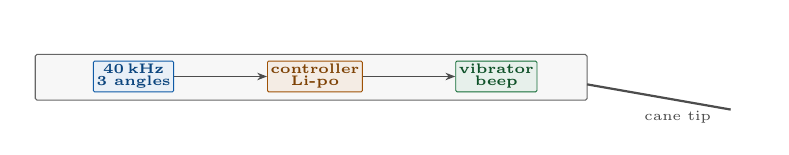
\begin{tikzpicture}[x=0.96mm,y=1mm]
  \draw[box,fill=black!3] (1,3.2) rectangle (74,9.0);
  \node[S] (us) at (14,6.2) {40\,kHz\\[-0.3mm]3 angles};
  \node[C] (mcu) at (38,6.2) {controller\\[-0.3mm]Li-po};
  \node[O] (vib) at (62,6.2) {vibrator\\[-0.3mm]beep};
  \draw[arr] (us) -- (mcu);
  \draw[arr] (mcu) -- (vib);
  \draw[line width=0.8pt,black!70] (74,5.2) -- (93,2.0);
  \node[lbl] at (86,1.0) {cane tip};
\pgfresetboundingbox\useasboundingbox (0,-0.2) rectangle (97,12.4);\end{tikzpicture}%
}
{Knee to head only, about a \(45^\circ\) cone. Indoor 0.03--1.8\,m, outdoor 0.03--3\,m. The vibration pattern is the distance; long mode also beeps above 65\,dB. The 0 / 17.8 / 35.6\(^\circ\) turret, the beeper, and the 3\,m outdoor range are what this product adds to the 2007 patent.}
\hfill
\cell{6 \quad CN 114246767 A \textnormal{\fontsize{4.6}{5}\selectfont --- Hohai, cloud navigation glasses}}
{%
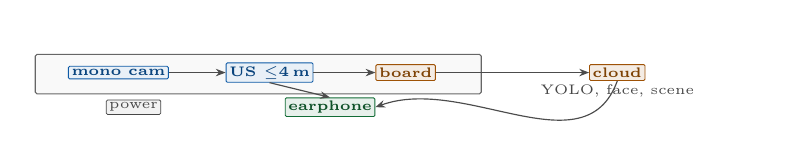
\begin{tikzpicture}[x=0.96mm,y=1mm]
  \draw[box,fill=black!2.5] (1,4.0) rectangle (60,9.0);
  \node[S] (cam) at (12,6.7) {mono cam};
  \node[S] (us) at (32,6.7) {US \(\le\)4\,m};
  \node[C] (bd) at (50,6.7) {board};
  \node[P] at (14,2.3) {power};
  \node[O] (ear) at (40,2.3) {earphone};
  \node[C] (cld) at (78,6.7) {cloud};
  \node[lbl] at (78,4.3) {YOLO, face, scene};
  \draw[arr] (cam) -- (us);
  \draw[arr] (us) -- (bd);
  \draw[arr] (bd) -- (cld);
  \draw[arr] (cld.south) to[out=-110,in=20] (ear.east);
  \draw[arr] (us.south) -- (ear.north);
\pgfresetboundingbox\useasboundingbox (0,-0.2) rectangle (97,12.4);\end{tikzpicture}%
}
{The 8\,MP camera uploads video over ZeroMQ. Ultrasound on the frame ranges obstacles the cloud cannot name. Cloud detection, face, scene, and monocular distance come back; the board turns them into one sentence. Speech synthesis runs in the cloud.}

\vspace{0.15mm}
\noindent
\cell{7 \quad SmartEye PathPal \textnormal{\fontsize{4.6}{5}\selectfont --- smart stick, offline}}
{%
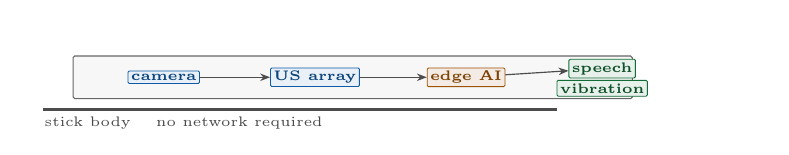
\begin{tikzpicture}[x=0.96mm,y=1mm]
  \draw[box,fill=black!3] (6,3.4) rectangle (80,8.8);
  \node[S] (cam) at (18,6.1) {camera};
  \node[S] (us) at (38,6.1) {US array};
  \node[C] (ai) at (58,6.1) {edge AI};
  \node[O] (out) at (76,7.2) {speech};
  \node[O] at (76,4.7) {vibration};
  \draw[arr] (cam) -- (us);
  \draw[arr] (us) -- (ai);
  \draw[arr] (ai) -- (out);
  \draw[line width=0.8pt,black!70] (2,2.0) -- (70,2.0);
  \node[lbl,anchor=west] at (2,0.3) {stick body \quad no network required};
\pgfresetboundingbox\useasboundingbox (0,-0.2) rectangle (97,12.4);\end{tikzpicture}%
}
{The camera and several ultrasonic axes feed models on the stick: objects, hanging obstacles, potholes and ledges, OCR, and currency. Speech and a distinct vibration pattern come back. It is meant for streets without a reliable connection.}
\hfill
\cell{7 \quad CN 113255483 A \textnormal{\fontsize{4.6}{5}\selectfont --- Xingyi, text / face / object}}
{%
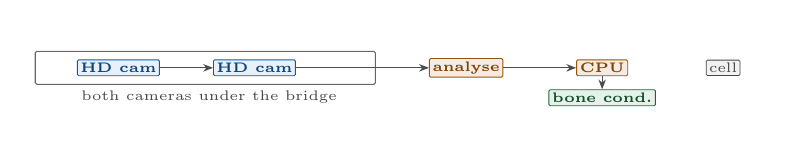
\begin{tikzpicture}[x=0.96mm,y=1mm]
  \draw[box] (1,5.2) rectangle (46,9.4);
  \node[S] (c1) at (12,7.3) {HD cam};
  \node[S] (c2) at (30,7.3) {HD cam};
  \node[C] (an) at (58,7.3) {analyse};
  \node[C] (cpu) at (76,7.3) {CPU};
  \node[O] (bc) at (76,3.5) {bone cond.};
  \node[P] at (92,7.3) {cell};
  \draw[arr] (c1) -- (c2);
  \draw[arr] (c2) -- (an);
  \draw[arr] (an) -- (cpu);
  \draw[arr] (cpu) -- (bc);
  \node[lbl] at (24,3.6) {both cameras under the bridge};
\pgfresetboundingbox\useasboundingbox (0,-0.2) rectangle (97,12.4);\end{tikzpicture}%
}
{Two cameras sit between the lenses. Capture, then analysis, then the CPU names text, a face, or an object. A voice module speaks it on a bone-conduction earphone. The side cable reaches the converter and the battery box.}

\vspace{0.7mm}
{\fontsize{4.15}{5}\selectfont\color{black!58}%
Layouts follow the published claims and specifications: Paul et al.\ and the Saksham SmartCane sheet; US 11,215,846 B1; US 2021/0390882 A1; US 12,044,541 B2; US 12,440,387 B2; CN 114246767 A; CN 113255483 A; OrCam and AFB; Envision / Glass EE2; Oculosense; WeWALK (MEMS ultrasonic ToF, two haptics, handle audio, Bluetooth phone); SmartEye PathPal; TSAR Labs' public page only.}
\end{document}
